A dust grain in the Solar system is a subject to many interactions. Grains of different sizes and in different locations are naturally susceptible to be influenced by different forces. In this chapter, we describe the most important forces and interactions, their causes and effects, as well as their relevance for different dust grains. We will later use this to discuss the properties and dynamics of dust populations in the Solar system. 

\section{Characterizing a single grain}

Newton's second law of motion has it, that
\begin{equation}
\vec{a} = \frac{\vec{F}}{m},
\end{equation}
where $\vec{a}$ is the acceleration of the object with the mass $m$, induced by the net force $\vec{F}$. Mass of a dust grain is related to its volume $V$ and the mean density of $\rho$ as
\begin{equation}
    m = V \rho.
\end{equation}
The mean density depends on the composition and the structure of the grain. 

\subsubsection{Dust composition}

Dust grains are relatively hard to collect, and they are mostly collected in the atmosphere of or in the near vicinity of the Earth. Some collection methods, such as collection in antarctic ice or from the deep see sediments \citep{brownlee1985cosmic} and the near ground collection \citep{pettersson1958rate} or the collection in the high atmosphere \citep{fechtig1968results} provided useful data, but are limited to specific dust grains, small and slow enough not to ablate in the atmosphere \cite{vondrak2008chemical}. These measurements are also challenging to be performed reliably, as they are very prone to contamination with terrestrial dust \citep{taylor2016cosmic}. 

Among the most valuable data points available to this date are the ones provided by the \textit{Space Shuttle} samples \citep{mcdonnell1984cosmic} and \textit{Stardust} cometary dust samples \citep{brownlee2014stardust}, both collected in aerogel \citep{tsou1995silica}. The samples returned from the vicinity of the \textit{Wild 2} comet were found to contain many elements, mostly silicon (\textit{Si}), magnesium (\textit{Mg}), iron (\textit{Fe}), and sulfur (\textit{S}) \citep{keller2006infrared}. Another proxy for the dust composition with much better data availability is the composition of meteorites. Among minerals typically found in meteorites are \textit{olivine}, \textit{quartz}, and \textit{pyroxenes}. Therefore, the most abundant elements in meteorites are again: \textit{Si}, \textit{Mg}, \textit{Fe}, and \textit{S}, but meteorites also show a vast variety and richness of composition \citep{anders1964origin} and there is therefore little doubt, that so does the interplanetary dust. 

The dust grains don't need to be collected for the composition analysis. A time-of-flight (\textit{ToF}) spectroscopy of dust was performed in the vicinity of the comet \textit{Halley} several times \citep{jessberger1988aspects}, which besides hydrogen (\textit{H}) and oxygen (\textit{O}) revealed mostly carbon (\textit{C}), \textit{Si}, \textit{Mg}, and \textit{Fe}. Optical measurements of the elemental abundance in the local interstellar cloud (LIC) also probes the dust composition. It shows a relative depletion of \textit{Si} and \textit{Mg}, which suggests these are bound in the dust grains present in the LIC. 

Based on several pieces of observational evidence, it is reasonable to assume that among the dominant constituents of the dust are \textit{H}, \textit{O}, \textit{Si}, \textit{Mg}, \textit{Fe}, and \textit{S}.

\subsubsection{Dust shape}

The shape of the grains is difficult to establish, since even the grains collected in aerogel are partially damaged during the collection \citep{burchell2006cosmic}. The grains collected in the upper atmosphere, on the sea floor and in deep ice were studied for their shape \citep{jessberger2001properties}, but the aforementioned difficulties with the selection bias prevail. A grain recovered from high atmosphere is shown in \Figref{fig:dust_grain}. Information on the dust shape is also yielded from the comparison of remote measurement of scattering properties with the models \citep{min2005modeling}. A lot was successfully achieved with modelling the dust grains are spheres or ellipsoids \citep{mann2010interstellar}, and for many modelling applications, the shape is not crucial.

\begin{figure}[h]
 	\centering
 	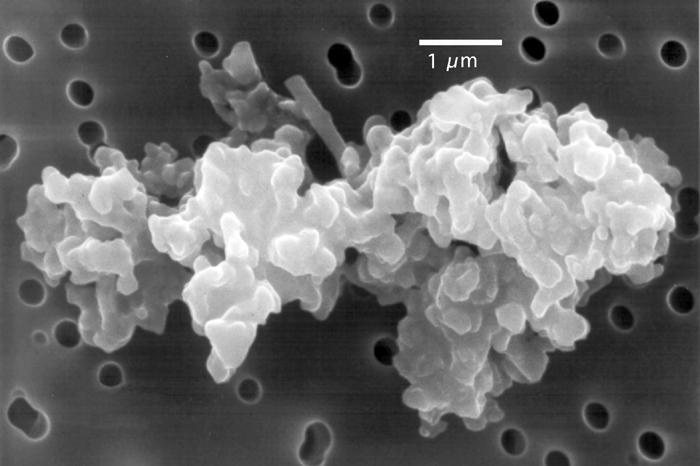
\includegraphics[width=8cm]{figures/grain.jpg}
 	\caption{A scanning electron microscopy (\textit{SEM}) image of a porous chondrite dust grain recovered from high atmosphere.  The authors of this figure are Donald E. Brownlee, University of Washington, Seattle, and Elmar Jessberger, Institut für Planetologie, Münster, Germany.
This file is licensed under CC-BY 2.5 License.}
 	\label{fig:dust_grain}
\end{figure}

\subsubsection{Dust density} \label{sec:density}

Bulk density of the common minerals containing the usual meteorite component elements, such as olivine, quartz or pyroxenes is between $2.6 \, \si{g cm^{-3}}$ and $3.8 \, \si{g cm^{-3}}$ \citep{duda1986minerals}. A lot of interplanetary dust contains ice, which naturally has a bulk density close to $1 \, \si{g cm^{-3}}$.

The density is often assumed between $2.5 \, \si{g cm^{-3}}$ \citep{mann2014dust} and $3 \, \si{g cm^{-3}}$ \citep{mcdonnell1984cosmic}. Dust grains are often, due to photometric and historical reasons described in terms of their linear dimension $d = 2r$, which more often than not means the diameter of the sphere with the volume $V$ equivalent to the dust grain's, hence
\begin{equation}
    d = 2 \left( {\frac{3V}{4\pi}} \right)^{\frac{1}{3}} \approx 1.24 \sqrt[3]{V}.
\end{equation}
Since we meet both mass-based notation and size-based notation, it is useful to keep the conversion in mind, which stands
\begin{equation}
    m = \rho \frac{4\pi}{3} r^3 = \rho \frac{\pi}{6} d^3 \Leftrightarrow d = \sqrt[3]{\frac{6 m}{\rho \pi}},
    \label{eq:density}
\end{equation}
and assuming $2.5 \, \si{g cm^{-3}}$ gives
\begin{equation}
    \frac{m}{\si{kg}} \approx 1.3 \cdot 10^3 \left(\frac{d}{\si{m}}\right)^3 
\Leftrightarrow 
    \frac{d}{\si{m}} = 9 \cdot 10^{-2} \sqrt[3]{\frac{m}{\si{kg}}},
\end{equation}
which is shown in \Figref{fig:mass_size_ruler}.

\begin{figure}[h]
 	\centering
 	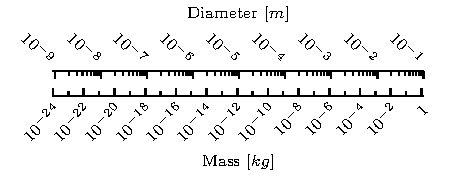
\includegraphics[width=10cm]{figures/mass_size_ruler.pdf}
 	\caption{A conversion between the mass and the diameter of a spherical dust grain, assuming the density of $2.5 \, \si{g cm^{-3}}$.}
 	\label{fig:mass_size_ruler}
\end{figure}

\section{Forces} 

\subsection{Gravity} \label{ch:gravity}

Gravity is an attractive pair force between two massive objects of the magnitude of 
\begin{equation}
    F_g = G \frac{M m}{R^2} = \mu \frac{m}{R^2},
\end{equation}
where $G \approx 6.67 \cdot 10^{-11} m^3 kg^{-1} s^{-2}$ is the \textit{gravitational constant}, $R$ is the distance between the objects' centres of mass, and masses $M$ and $m$ belong, by convention, to the more and less massive of the objects, respectively. Alternatively, $\mu = G M$ is known as the \textit{gravitational parameter}, which provides a convenient form for the force, especially if $m \ll M$, as is certainly the case of dust grains, with respect to planets and the Sun. In case of the Sun, $\mu \approx 1.3 \cdot 10^{20} \si{m^3 s^{-2}}$.

Due to the steep dependence of the force on the distance $F_g \propto R^{-2}$, it is often the case that a single central body suffices to describe the net gravity force affecting a smaller body. This concept is known as the \textit{Hill sphere}, which is the sphere of influence around every body in the Solar system, within which the body's gravity is the most relevant contributor to the net gravity, compared against the gravity of the Sun. The approximate planet's Hill radius is equal to the distance to the $L_1$ or the $L_2$ Lagrange point, therefore 
\begin{equation}
    R_H \approx a \sqrt[3]{\frac{m}{3M}},
\end{equation}
where $a$ is the planet's semimajor axis, $m$ is the mass of the planet, and $M$ is the mass of the Sun \cite{sheppard2023new}. For example, Saturn's Hill sphere with the Hill radius of $R_{H;Saturn} \approx 0.4 \, \si{AU}$ is necessary for Saturn to retain is $146$ confirmed moons \citep{sheppard2023new}, as well as its far reaching rings. The rings are an example of a dust system bound to a planet. The Sun is however by far the dominant object in most of the Solar system, especially within $1 \, \si{AU}$, and its gravity is usually the only one that is relevant for the dust grain in question.

Object orbit the Sun on circular orbits, if the magnitude of centrifugal force $F_c$ is equal to the magnitude of gravity $F_g$. This condition gives the \textit{circular speed} $v_c$ needed for the equality: 
\begin{equation}
    \frac{m v_c^2}{R} = \mu \frac{m}{R^2} \Leftrightarrow v_c = \sqrt{\frac{\mu}{R}} \Leftrightarrow R = \frac{\mu}{v_c^2}.
    \label{eq:circular_speed}
\end{equation}
The circular speed $v_c$ at $R = 1 \, \si{AU}$ is $v \approx 29.8 \, \si{km s^{-1}}$. Since gravity ceases with $R \to \infty$ as $F_g \propto R^{-2}$, the work needed in order to escape a gravity well is finite. The minimum energy sufficient for the escape is provided by the \textit{escape speed} $v_e$: 
\begin{equation}
    \frac{m v_e^2}{2} = \frac{\mu m}{R} \Leftrightarrow v_e = \sqrt{\frac{2 \mu}{R}} = \sqrt{2} v_c.
    \label{eq:escape_speed}
\end{equation}

\subsection{Radiation pressure}

The power density of solar radiation at $1 \si{AU}$ is $G_{SC} \approx 1361 \, \si{W m^{-2}}$ \citep{kopp2011new} and corresponds to the radiative power of the Sun $P_{Sun} \approx 3.9 \cdot 10^{26} \, \si{W}$. Dividing $G_{SC}$ by the speed of light $c \approx 3\cdot10^8 \, \si{m s^{-1}}$ gives the radiation pressure of
\begin{equation}
    p_{rp}(1 \si{AU}) = \frac{G_{SC}}{c} \approx 4.5 \cdot 10^{-6} \, \si{Pa},
    \label{eq:radiation_pressure}
\end{equation}
and the resulting radiation pressure force $F_{rp}$ is readily obtained as
\begin{equation}
    F_{rp} = p_{rp} S = \frac{P_{Sun}}{4 c \pi R^2} S = \frac{P_{Sun}}{cR^2} r^2, \label{eq:radiation_pressure_force}
\end{equation}
where $S$ is the Sun-facing cross section of the body of interest, $r$ is the body's radius, and $R$ is the distance of the body from the Sun, whereas in the second equation we also assumed the body to be spherical and the Sun to be a point source: $r \ll R$. A dimensionless parameter $\beta$ is used to describe the relative importance of the two forces:
\begin{equation}
    \beta = \frac{F_{rp}}{F_g}.
\end{equation}
Since $F_{rp}$ directly opposes $F_g$, the net force, denoted \textit{effective gravity}, or $F_{eg}$ is obtained as
\begin{equation}
    F_{eg} = F_g - F_{rp},
\end{equation}
and using $\beta$, we get
\begin{equation}
    F_{eg} = (1-\beta) F_g.
\end{equation}
In the case of the Earth, the radiation pressure force is $F_{rp;Earth} \approx 5.8 \cdot 10^8 \, \si{N}$, which might be compared to the gravity between the Earth and the Sun $F_{g;Earth} \approx 5.2 \cdot 10^{33} \si{N}$, resulting in $\beta_{Earth} \approx 10^{-25}$. 

Interestingly, both $F_g$ and $F_{rp}$ scale with the distance from the Sun as $F \propto {R^{-2}}$, as long as the Sun is assumed a point source of radiation. Therefore, $\beta$ is not a function of the distance from the Sun $R$, and we are permitted to express the effective gravity as 
\begin{equation}
    F_{eg} = (1-\beta) G \frac{M m}{R^2} = (1-\beta) \mu \frac{m}{R^2} = \mu_{e} \frac{m}{R^2},
    \label{eq:effective_gravity}
\end{equation}
where $\mu_{e}$ is the body-specific effective gravitational parameter, taking radiation pressure into account. We see that the laws of orbital motion (for example Eqs. \ref{eq:circular_speed} and \ref{eq:escape_speed}) of radiation pressure affected bodies are going to be the same, albeit with a different gravitational parameter $\mu_e$.

We found that $\beta$ only depends on the properties of the Sun and the body in question, and is therefore body specific. Let us study the dependence of $\beta$ on the size of the body in question $r$. It follows that as long as the aforementioned equations for $F_{g}$ and $F_{rp}$ hold, $\beta$ depends on $r$ as 
\begin{equation} 
    \beta = \frac{\frac{P_{Sun}}{c R^2} r^2}{\mu \frac{m}{R^2}} = \frac{P_{Sun}}{\mu c} \frac{r^2}{\rho V} = \frac{P_{Sun}}{\mu c \rho} \frac{3 r^2}{4 \pi r^3} = \frac{3 P_{Sun}}{4 \pi \mu c \rho} r^{-1},
\end{equation}
therefore $\beta \propto r^{-1}$, which is not surprising, given $F_{g} \propto m \propto r^{3}$ and 
$F_{rp} \propto S \propto r^{2}$. Assuming the density of $\rho \approx 2.5 \si{gcm^{-3}}$ as in Sec. \ref{sec:density}, we find that 
\begin{equation}
    \beta \approx 9.6 \cdot 10^{-7} r^{-1} \, \si{m},
    \label{eq:beta_estimate}
\end{equation}
which gives that for $\beta = 1$, that is the radiation pressure force offsetting the gravity fully, the dust grain has to have the radius of $r \approx 960 \, \si{nm}$. However, Eq. \eqref{eq:radiation_pressure_force} assumes the solar photons are either absorbed, or scattered fully as a spherical wave with their momentum transferred to the body. This holds for absorbing materials if $r \gg \lambda$, where $\lambda$ is the wavelength of the radiation. However, $r \approx 950 \si{nm}$ is comparable to the typical sunlight photons and the assumption does not hold fully. A proper calculation of light scattering is necessary and it depends on the material and shape of the grain. This was done previously by other authors \cite{kimura2003composition} for reasonable materials, see Fig. \ref{fig:kimura_mie}. It was found that the maximum of $\beta$ is reached between $10^{-17} - 10^{-16} \si{kg}$, which corresponds to the diameter of $100 - 300 \si{nm}$, depending on the material. In any case, the maximum value of $\beta$ is on the order of unity and lower than unity for much smaller or larger grains.

\begin{figure}[h]
 	\centering
 	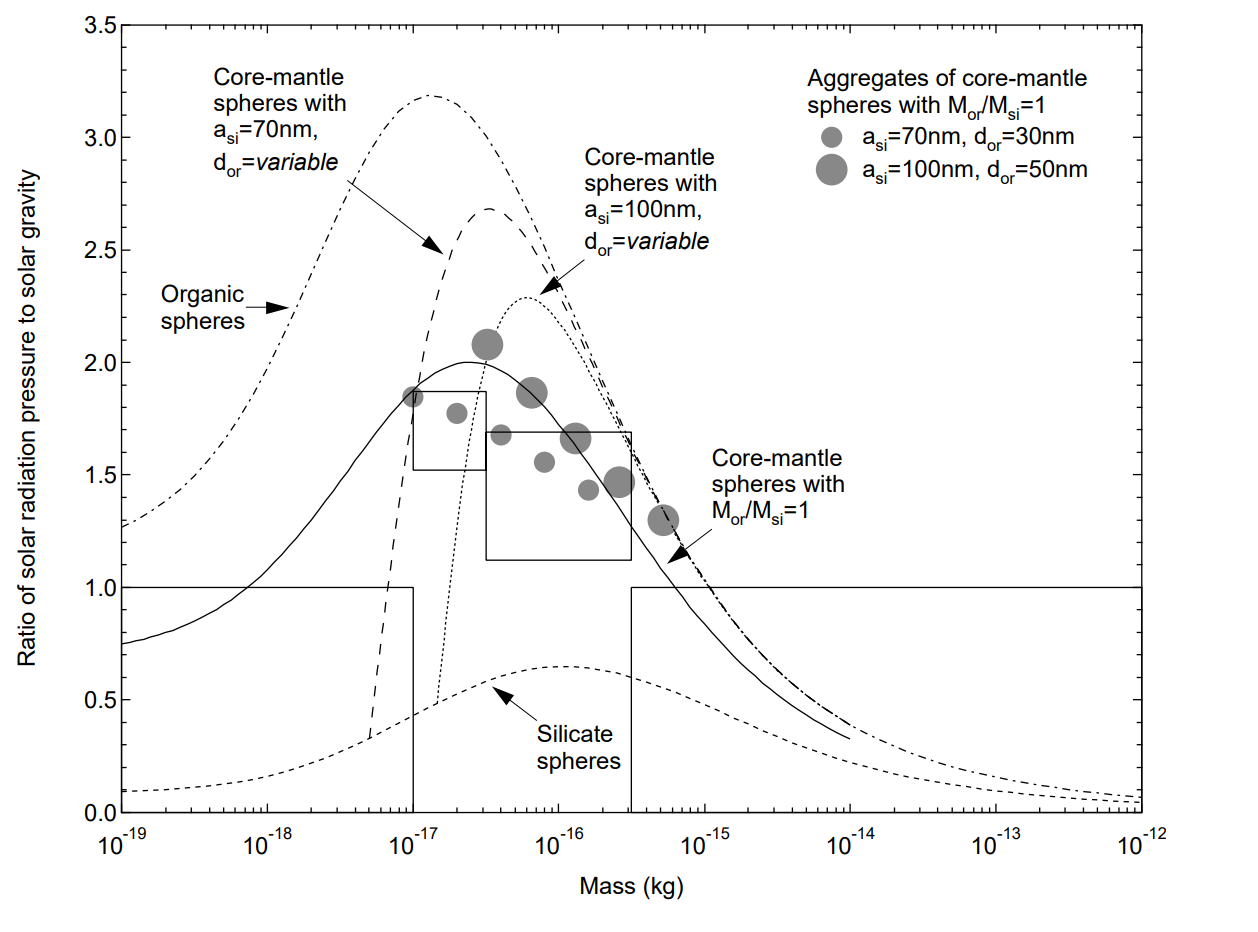
\includegraphics[width=10cm]{figures/kimurra_mie.png}
 	\caption{The light scattering calculation result for the $\beta$ value (\textit{y}-axis) as a function of mass of spherical grains of various composition, adapted from \cite{kimura2003composition}.}
 	\label{fig:kimura_mie}
\end{figure}

\subsection{Lorentz force}

\subsubsection{Grain's potential}

The grains in the solar system are immersed in the ambient plasma and subjected to the solar UV irradiation, both of these causing charging of the grains. Should the ambient conditions remain stable, the grain's electric charge reaches equilibrium. The main charging currents are \textit{electron collection current} and the \textit{photoemission current}. They act to charge the grain to a negative and positive potential respectively. Should the plasma be dense or should the grain be in shadow, the former prevails and the grain's potential becomes negative. Should the plasma be sparse and the UV irradiation dense, the latter prevails and the grain becomes positively charged. We will now examine the two extreme cases. 

An object immersed in plasma charges to so-called \textit{floating potential}. This potential $\phi_{f}$ is typically negative, which is a result of the electron mobility being much higher, compared to the ion mobility. The charging current ceases if the potential of the grain poses a significant barrier to the electrons, therefore the maximum potential is on the order of electron temperature $T_e$, which is approximately $8 \, \si{eV k_B^{-1}}$ near $1 \, \si{AU}$ and $20 \, \si{eV k_B^{-1}}$ near $0.25 \, \si{AU}$ in the typical solar wind \citep{guillemant2013simulation}. 

Electrons are released from an illuminated neutral grain, in case the incident photon's energy $h\nu$ is above the photoelectric work function $W_{p}$ of the grain material. This typically requires UV photons and leaves the grain more positively charged, which adds additional barrier for the next photoelectron to surpass. The established positive potential $\phi_{p}$ is such that no more electrons can escape, therefore it is $\phi_{p} \approx h\nu - W_{p}$. While $W_p$ for common materials is between $2 - 5 \, \si{eV}$, the last strong spectral line of she sunlight is \textit{Ly-$\alpha$} at $h\nu \approx 10.2 \, \si{eV}$, resulting in the maximum potential of $\phi_p$ between $5 - 8 \, \si{V}$. 

The equilibrium potential $\phi$ of the grain depends on the ambient plasma conditions and the properties of the grain, but typically settles on a value between $-20 \, \si{V}$ and $+8 \, \si{V}$. A more comprehensive and careful study is out of scope of this work, but is found in literature \citep{meyer1982flip,horanyi1996charged,krivov1998dynamics,dzhanoev2016charging,vaverka2016lunar}.

\subsubsection{Grain's charge}

An isolated grain's charge $q$ is related to its potential $\phi$ as
\begin{equation}
    q = C \phi, \label{eq:charge}
\end{equation}
where $C$ is the grain's capacitance. The capacitance of a solitary sphere in vacuum with the radius of $r$ is 
\begin{equation}
    C_{sphere} = 4 \pi \epsilon_0 r,
\end{equation}
which translates using Eq. \ref{eq:charge} to
\begin{equation}
    \frac{q}{r \phi} = 4 \pi \epsilon_0 \approx 1.1 \cdot 10^{-10} \, \si{C V^{-1} m^{-1}},
    \label{eq:capacitance}
\end{equation}
where $\epsilon_0 \approx 8.9\cdot10^{-12} \, \si{C V^{-1} m^{-1}}$ is the free space permittivity. This simplistic model predicts the charge of $\pm 10^{-15} \, \si{C}$ for a spherical grain with the radius of $r = 1 \, \si{\mu m}$ at the potential of $\phi = \pm 9 \, \si{V}$. We note that this value is order of magnitude correct for a grain of arbitrary shape with the greatest linear extent of $\approx 2r$. 
The ratio of mass $m$ to charge $q$ is relevant for the dynamics of dust grains. Given the charge as in Eq. \ref{eq:capacitance}, and the mass as in Eq. \ref{eq:density}, we get
\begin{equation}
    \frac{q}{m} = \frac{3 \epsilon_0 \phi}{\rho r^2} \approx 10^{-13} r^{-2} \, \si{m^2},
    \label{eq:charge_estimate}
\end{equation}
where we assumed $\phi \approx 9 \, \si{V}$ and the bulk density $\rho \approx 2.5 \, \si{g cm^{-3}}$ as before. Eq. \ref{eq:charge_estimate} is visualized in Fig. \ref{fig:charge_density_ruler}.

\begin{figure}[h]
 	\centering
 	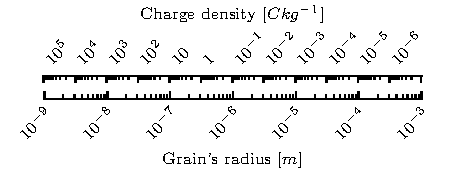
\includegraphics[width=10cm]{figures/charge_density_ruler.pdf}
 	\caption{A conversion between the radius $r$ and the charge density $q/m$ as in Eq. \ref{eq:charge_estimate}.}
 	\label{fig:charge_density_ruler}
\end{figure}

\subsubsection{Dynamics}

A point charge is usually a very suitable model for a charged dust grain. The Lorentz force acting on a point charge $q$ is
\begin{equation}
\vec{F}_{EM} = q \left( \vec{E} + \vec{v} \times \vec{B} \right),
\end{equation}
where $\vec{E}$ and $\vec{B}$ are the ambient electric and magnetic fields respectively, and $\vec{v}$ is the velocity of the point charge. If the charge $q$ is sufficient, $F_{EM}$ might be more important than effective gravity:
\begin{equation}
    F_{eg} < F_{EM} \Rightarrow \frac{q}{m} > \frac{(1-\beta)\mu}{R^2 \left| \vec{E} + \vec{v} \times \vec{B} \right|}. \label{eq:lorentz_gravity}
\end{equation}
As an order of magnitude estimate, let's assume 
\begin{equation}
    F_{EM} \approx q v_{sw} B_{IMF},
\end{equation}
in addition to $\beta = 0$ and $B_{IMF} = 4 \, \si{nT}$, which is a reasonable magnetic field strength near $R = 1 \, \si{AU}$ \citep{mann2007nanoparticles}. This places the condition \ref{eq:lorentz_gravity} to
\begin{equation}
    \frac{q}{m} > 5 \, \si{C kg^{-1}},
\end{equation}
which translates using Eq. \ref{eq:charge_estimate} to $r < 0.14 \, \si{\mu m}$, and is not very sensitive to $R$, provided that $B \propto R^{-2}$, which can often be assumed if $R \gg R_{Sun}$ \citep{parker1958dynamics}.  

This condition describes the state in which Lorentz force is grater in amplitude than gravity. If they are comparable, the curvature in the trajectory of the dust grain due to Lorentz force is similar to the curvature of the trajectory due to the force of gravity, which is on the Solar system scale. We therefore must consider the temporal aspect: given enough time, even $F_{EM} \ll F_g$ might be consequential for the motion of the dust grain, and, vice-versa, $F_{EM} \approx F_g$ does not imply that the grain does not move along a straight line when inspected locally. 

Eq. \ref{eq:lorentz_gravity} has many degrees of freedom. The ratio of $q/m$ is the most important of the grain's properties and the grain's motion is often studied with respect to its $q/m$. \citeauthor{czechowski2010formation} \citep{czechowski2010formation} studied the motion of charged grains released in the vicinity of the Sun with the circular speed and charge density of about $10^3 \, \si{C kg^{-1}}$, which corresponds to the radius of $r \approx 10 \, \si{nm}$. The assumed the magnetic field $\vec{B}_{IMF}$ is was described by the Parker spiral \citep{parker1958dynamics} with tilted heliospheric current sheet (\textit{HCS}). They found that if the grains are produced within $0.15 \, \si{AU}$, they remain trapped near the Sun, on non-keplerian orbits with very low aphelia, and therefore are likely destroyed. If the grains are produced outside of $0.2 \, \si{AU}$, they are expelled outward, and their velocity at $1 \, \si{AU}$ depends on their $q/m$, and is on the order of $200 \, \si{km s^{-1}}$ if $q/m \gtrsim 10^3 \, \si{C kg^{-1}}$, and lower for grains with lower $q/m$. 

The motion of dust near the Sun was studied theoretically by other authors, and many effects were described, such as inclination increase \citep{krivov1998dynamics}, ejection \citep{krivov1998dynamics}, and gradual shift of the dust cloud symmetry plane \citep{morfill1979motion}.

\citeauthor{poppe2020effects} \cite{poppe2020effects} studied variability of the flux of dynamically charging $\si{nm}$-sized grains. They made use of electromagnetic field given by a time variable, semi-empirical, corona-solar wind coupled model and found strong variability in the distribution of grains arriving at $1 \, \si{AU}$ within one Carrington rotation. Especially grains with the radius $r<10 \, \si{nm}$ were found to arrive at $1 \, \si{AU}$ with the speed well correlated with the local solar wind speed $v_{sw}$. 

Numerous other publications studied motion of charged grains immersed in the solar system plasma \citep{mann2007nanoparticles,horanyi1996charged,juhasz2013dynamics,stamm2019dust,czechowski2021dynamics,poppe2022effects,rusk1988effect}.

\subsection{Poynting-Robertson drag} \label{ch:pr_drag}

Since an object orbiting the Sun is moving with respect to the source of radiation, the position of the Sun as seen from the object is apparently different, \textit{aberrated}, by an angle of the order of $v/c$, where $v$ is the orbital speed of the object, and $c$ is the speed of light. Therefore, the light doesn't come from pure radial direction, but partially from from the \textit{ram direction}, as observed from the orbiting object. The scattering and absorption of the light then leads to a negative change in the momentum, and therefore in the orbital speed \citep{poynting1903radiation}. The magnitude of Poynting-Robertson effect is \citep{robertson1937dynamical}:
\begin{equation}
    F_{PR} = \frac{v}{c^2} P_{r},
    \label{eq:poynting_robertson}
\end{equation}
where $P_r$ is the power of incoming solar radiation assuming the object's cross section $S$: 
\begin{equation}
    P_{r} = \frac{P_{Sun} S}{4 \pi R^2}.
    \label{eq:radiation_power}
\end{equation}
Assuming the object is on a circular orbit, we make use of Eqs. \ref{eq:poynting_robertson}, \ref{eq:circular_speed}, and \ref{eq:radiation_power} to get
\begin{equation}
    F_{PR} = \sqrt{\frac{\mu}{R}} \frac{P_{r}}{c^2} = \frac{P_{Sun}S}{4 \pi c^2} \sqrt{\frac{\mu}{R^5}}. 
\end{equation}
As an estimate of magnitude of $F_{PR}$, we evaluate the effective pressure $p_{PR}$:
\begin{equation}
    p_{PR} = \frac{F_{PR}}{S} = \frac{P_{Sun}}{4 \pi c^2} \sqrt{\frac{\mu}{R^5}} \approx 4.5 \cdot 10^{-10} \, \si{Pa},
\end{equation}
where we assumed $R \approx 1 \, \si{AU}$, and $c$, $P_{Sun}$, and $\mu$ as before.

As an estimate of relevance of $F_{PR}$, we may study the dynamic evolution of the orbital speed, and, by extension, orbital radius. Although $F_{PR}$ acts against the speed $v$, the speed will actually be rising, as lower energy implies higher orbital speed. Eq. \ref{eq:poynting_robertson} gives for the acceleration $a$ in time
\begin{equation}
    a_{PR}(t) = \frac{dv}{dt}(t) = \frac{P_{r}(t)v(t)}{mc^2} = \frac{P_{Sun} v(t) }{4 \pi R^2(t) c^2} \frac{S}{m},
\end{equation}
where we use the assumption of circularity (Eq. \ref{eq:circular_speed}) once again to get
\begin{equation}
    a_{PR}(t) = \frac{P_{Sun}}{4 \pi \mu^2 c^2} \frac{S}{m} v^5(t),
\end{equation}
which is separable with a single positive real solution for $v(t)$:
\begin{equation}
    v(t) = \left( v(0)^{-4} - \frac{P_{Sun}}{\pi \mu^2 c^2} \frac{S}{m} t \right)^{-\frac{1}{4}},
\end{equation}
which translates to $R$:
\begin{equation}\begin{split}
    R(t) &=  \mu \sqrt{ \left(\frac{R_0}{\mu}\right)^{2} - \frac{P_{Sun}}{\pi \mu^2 c^2} \frac{S}{m} t }
    \\ &= \sqrt{R_0^2 - \frac{P_{Sun}}{\pi c^2} \frac{S}{m} t }.
\end{split}\end{equation}
Assuming a spherical dust grain (Eq. \ref{eq:density}), we get
\begin{equation}
    R(t) = \sqrt{R_0^2 - \frac{P_{Sun}}{\pi c^2} \frac{\pi r^2}{\rho \frac{4\pi}{3} r^3} t } = \sqrt{R_0^2 - \frac{3P_{Sun}}{4 \pi \rho c^2} \frac{t}{r} },
    \label{eq:PR_estimate}
\end{equation}
where the factor of $t/r$, the time-scale of the orbital evolution, is proportional to the grain's linear size. Assuming $P_{Sun},\rho$ as before, $r=1\,\si{\mu m}$ grain will spiral from $R_0=1\,\si{AU}$ down to $R=0.1\,\si{AU}$ in $t=1.7 \cdot 10^3\,\si{yr}$. This time becomes $10^6\,\si{yr}$ if we assume an object with the radius of $r \approx 0.6 \, \si{m}$, therefore $F_{PR}$ is irrelevant for the dynamics of macroscopic object, but relevant for the dynamics of the Solar system's dust cloud. 

We note that circular orbits subjected to $F_{PR}$ remain circular. Briefly, and without mathematical rigor, deceleration in the perihelion does not change the perihelion distance $r_{peri}$, but lowers the aphelion distance $r_{aph}$. This decreases eccentricity $e$. Correspondingly, deceleration in the aphelion lowers $r_{peri}$, doesn't change $r_{aph}$ and therefore increases eccentricity. We note that $F_{PR} \propto v P_r$, and both these factors reach their maximum in the perihelion of an eccentric orbit, and their minimum in the aphelion, therefore eccentricity is gradually reduced and circular orbit's $e=0$ is stable. Rigorous results for non-circular orbits are available in the literature \cite{wyatt1950poynting}. 

\subsection{Solar wind pressure}

Interplanetary dust grains are in interaction with the solar wind plasma. The solar wind particles are in predominantly radial motion and they therefore project radial pressure $p_{sw}$ on the dust grains, which is in case of a stationary dust grain easily estimated \citep{shue1998magnetopause} as
\begin{equation}
    p_{sw} = n m_p v^2_{sw},  
\end{equation}
where $n$ is the number density of solar wind protons with mass $m_p$, $v_{sw}$ is the solar wind bulk speed, if only solar wind protons are considered and all the protons are assumed to fully pass ther momentum to the grain. Assuming typical $1 \, \si{AU}$ values of $v_{sw} \approx 300 \, \si{km s^{-1}}$, $n \approx 10^7 \, \si{m^{-3}}$, and $m_p \approx 1.67 \cdot 10^{-27} \, \si{kg}$, we get $p_{sw} \approx 1.5 \cdot 10^{-9} \, \si{Pa}$. We note that $p_{sw} \ll p_{rp}$ (see Eq. \ref{eq:radiation_pressure}). Since both pressures scale as $p \propto R^{-2}$ with the heliocentric distance $R$, solar wind pressure in radial direction $p_{sw}$ is typically negligible compared to the radiation pressure $p_{rp}$.

Even though radial effect of solar wind pressure is negligible compared to radiation pressure, its azimuthal component is not, since the orbital speed of a dust grain $v$ is much closer to the solar wind speed $v_{sw}$ than to the speed of light $c$. Considering a dust grain with speed $\vec{v} = \vec{e_r}v_r + \vec{e_\phi}v_\phi$, the force $\vec{F}_{sw} = \vec{e_r}F_{sw,r} + \vec{e_\phi}F_{sw,\phi}$ on the dust grain is \citep{burns1979radiation}
\begin{equation}\begin{split}
    F_{sw,r} &= S p_{sw} \left( 1-\frac{2v_r}{v_{sw}} \right), \\
    F_{sw,\phi} &= S p_{sw} \left( \frac{v_\phi}{v_{sw}} \right).
\end{split}\end{equation}
The force $F_{sw,\phi}$ is often called pseudo-Poynting-Robertson drag, since it acts similarly to $F_{PR}$ discussed in Sec. \ref{ch:pr_drag}. Assuming orbital speed of the Earth $v_\phi \approx 30 \, \si{km s^{-1}}$ and $v_{sw} \approx 300 \, \si{km s^{-1}}$, we find 
\begin{equation}
    p_{sw,\phi} = \frac{F_{sw,\phi}}{S} \approx 1.5 \cdot 10^{-10} \, \si{Pa},
\end{equation}
which is comparable to $p_{PR} \approx 4.5 \cdot 10^{-10} \, \si{Pa}$ at the same heliocentric distance $R = 1 \, \si{AU}$. With more careful treatment, it was estimated that $p_{sw,\phi} \approx 0.22 p_{PR}$ for typical dust grains \citep{whipple1967maintaining}, and more recently it was found that $p_{sw,\phi} > p_{PR}$ for certain grains with radii $r<0.1 \, \si{\mu m}$, and even $p_{sw} \approx p{rp}$ for silicate grains with radii $r<10 \, \si{nm}$, since the cross section with ions is much better than the cross section with sunlight photons for small particles \citep{mukai1982solar}. 

\section{Erosion} \label{ch:erosion}

The mass of a grain evolves abruptly at \textit{collisions} and gradually due to the solar radiaton and the ambient plasma. The solar radiation is responsible for \textit{sublimation}, while the plasma environment, namely solar wind, is responsible for \textit{sputtering}. 

\subsection{Sublimation}

To find under what conditions sublimation is important, we will examine the \textit{black body temperature}, that is the equilibrium temperature of an object in sunlight. We note that the temperature of a dust grain may, depending on the size and composition, differ from the black-body temperature by a factor of $3$, where the deviation is most prominent for grains with the radius $r \ll 1 \, \si{\mu m}$ \citep{myrvang2018temperature}, where scattering effect must be treated carefully. However, for larger grains of common material, the black body temperature is a useful approximation. 

The black body temperature in the vicinity of a star is obtained by comparing the incoming solar radiation $P_{r}$ (Eq. \ref{eq:radiation_power}) and the output power $P_{out}$ of the body:
\begin{equation}
    P_{out} = S_{tot} \sigma T^4,
    \label{eq:stefan_boltzmann}
\end{equation}
where $S_{tot}$ is the emitting surface of the body, $\sigma$ is the Stefan-Boltzmann constant, and $T$ is the temperature of the black body. Eq. \ref{eq:stefan_boltzmann} is the Stefan-Boltzmann law \citep{stefan1879uber,boltzmann1884ableitnung}. Comparing this to Eq. \ref{eq:radiation_power}, we get the condition for the power equality:
\begin{equation}
    \frac{P_{Sun} S}{4 \pi R^2} = S_{tot} \sigma T^4 \Leftrightarrow T =  \frac{1}{2} \sqrt[4]{\frac{P_{Sun}}{\sigma \pi}} \frac{1}{\sqrt{R}} \approx 279 \, \si{K} \left(\frac{R}{\si{AU}}\right)^{-\frac{1}{2}}, 
\end{equation}
where we note $S$ is the cross section of the grain, whereas $S_{tot}$ is the irradiating surface of the grain, and for a sphere $S_{tot} = 4S$. For reference, the melting point of iron is approxiamtely $1800 \, \si{K}$ and the melting point of olivine is between $1500 \, \si{K}$ and $2200 \, \si{K}$, depending on the exact composition \citep{liu1975melting,pinti2015olivine}. The relation as in the equation is shown in Fig. \ref{fig:black_body_temperature}, along with the melting point of water and the highest melting point of olivine.

\begin{figure}[h]
 	\centering
 	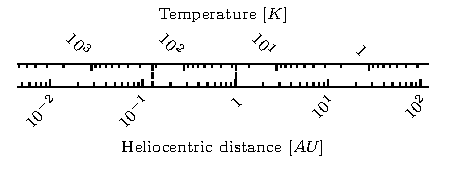
\includegraphics[width=10cm]{figures/distance_temperature_ruler.pdf}
 	\caption{The equilibrium black body temperature as a function of heliocentric distance, assuming spherical body. The temperatures of $273 \, \si{K}$ and $2200 \, \si{K}$ are shown for reference.}
 	\label{fig:black_body_temperature}
\end{figure}

The rate of sublimation of droplets is described by Langmuir's evaporation equation \citep{langmuir1918evaporation}:
\begin{equation}
    \frac{dm}{dt} = -p_{v} S_{tot} \sqrt{\frac{M_e}{2\pi RT}},
\end{equation}
where $p_v$ is the vapor pressure of the droplet fumes at the temperature of the droplets $T$, $S_{tot}$ is the surface of the droplet, $M_e$ is the molar mass of the fumes, and $R$ is the gas constant. This is applicable on dust grains composed of a sublimating material. The parameters $p_v$ and $M_e$ are material-dependent, and the former is also a steeply increasing function of $T$. We note the proportionality to $S_{tot}$, which implies that the sublimation lifetime is proportional to the original radius $r$ of a spherical grain. The differential equation can be solved for initial dust composition and temperature.   

\subsection{Sputtering}

Sputtering is a non-thermal process of erosion of an object due to collisions between the object and energetic particles. Unlike sublimation, sputtering depends on the properties of the plasma environment in addition to the properties of the bombarded object. In the Solar system, the energetic particles are provided by the Sun, in the form of \textit{solar wind} and occasional mass ejections. Sputtering mass loss rate is measured in laboratory as
\begin{equation}
    \frac{dm}{dt} = - \frac{ M_e S \lambda_i Y }{N_A}, 
    \label{eq:sputtering}
\end{equation}
where $M_e$ is the molar mass of the grain's atoms, $S$ is the grain's cross section, $\lambda_i$ is the flux of incident particles, $N_A$ is Avogadro's constant and finally $Y$ is the dimensionless \textit{sputtering yield}, which is modelled as a function of the state of the grain, and energy and mass of the incident particles \citep{vyvsinka2018odpravsovani}. Many assumptions must be done in order to solve the differential equation \ref{eq:sputtering}. 

\subsection{Collisions} \label{ch:collisions}

High-speed collisions between dust grains are inelastic and the mass distribution is changed as the parent grains produce smaller offspring grains. Assume the parent grains have masses $M_1$ and $M_2$, where $M_1 < M_2$. Modelling success was previously achieved \citep{gault1963spray,dohnanyi1969collisional} by assuming so-called \textit{crushing law} to be of the form
\begin{equation}
    g(m) = C(M_1,M_2)m^{-\eta},
    \label{eq:crushing_law}
\end{equation}
where $g(m)$ is a probability density function for the offspring mass $m$, $\eta$ is the power-law exponent, and the factor $C$ is a function of the parent objects' masses. Since the power-law distribution is constrianed by the total amount of collisionally ground material $M_\Sigma$ and is right-bound due to the upper limit of the offspring grain mass $M_{max}$ (that is the largest offspring grain), the normalization is
\begin{equation}
    C(M_1,M_2) = (2-\eta) M_\Sigma M_{max}^{\eta -2}.
\end{equation}
The parameter of $\eta$ was experimentally established \citep{gault1963spray} to be $\eta \approx 1.8$, in case $M_2 \rightarrow \infty$ which implies that most of the offspring mass is retained in the small offspring grains. 
A related modelling concept is that of \textit{catastrophic collisions} \citep{dohnanyi1969collisional,grun1985collisional}. These are collisions which completely shatter both parent grains: $M_\Sigma = M_1 + M_2$. If the smaller of the grains is too small $M_1 \ll M_2$, the bigger grain is not shattered completely. Laboratory experiments have repeatedly shown linearity of the process in mass \citep{gault1963spray,dietzel1973heos,grun1984impact,mcbride1999meteoroid,collette2014micrometeoroid,shen2021cosmic}. In that case, the condition for a catastrophic collision can be written as 
\begin{equation}
    M_2 < \Gamma M_1,
\end{equation}
where the threshold ratio $\Gamma$ is a theoretical concept only, and is a decreasing function of the impact speed and a function of the material properties. It is also difficult to establish experimentally \citep{grun1985collisional}, and different values are found in the literature. For the impact speed of $10 \, \si{km/s}$, the values on the order of $5 \cdot 10^{4}$ were reported \citep{gault1969destruction,fujiwara1977destruction}, but they range from $10^2$ to $5\cdot 10^5$ for broader speed interval \citep{whipple1967maintaining,zook1975source,dohnanyi1978particle}. 
Collisional lifetime of a dust grain is the time it takes for this test dust grain to catastrophically collide with another. This other grain is likely to be smaller than the test grain, since there are many more (by count) small dust grains than large dust grains. Collisional lifetime greatly depends on the mass and speed distribution and to some extent also on the material properties of the dust grains, and is therefore dependent on the heliospheric region. 

\subsection{Lifetimes}

All three erosion processes presented in this section (sublimation, sputtering, and collisions) depend, beyond other assumptions, on the size, the material, and on the location in the Solar system. All three are major factors in shaping the solar system dust cloud's dynamics and are important in different heliocentric regions. 

It was reported that for the dust of radius $r \approx 1 \, \si{\mu m}$, the collisional lifetime at $1\,\si{AU}$ is on the order of $10^6 \, \si{yr}$, whereas at $0.1\,\si{AU}$ it is on the order of $10^3 \, \si{yr}$ \citep{grun1985collisional}. We can compare this to the sputtering lifetime of silicate grains of the same size, which was calculated to be much shorter at  $\approx 10^4 \, \si{yr}$ at $1\,\si{AU}$, and $\approx 10^2 \, \si{yr}$ at $0.1\,\si{AU}$ even in slow solar wind conditions \citep{klepper2021influence}. It was in fact calculated \citep{klepper2021influence} that the sputtering lifetime is shorter than collisional lifetime between $0.1 \, \si{AU}$ and $1 \, \si{AU}$ for silicate and metal oxidee dust grains with $r<20 \, \si{\mu m}$.

Due to its speed dependence on the grain's temperature, sublimation prevails in the near vicinity of the Sun. It was evaluated to be dominant within $R < 0.1 \, \si{AU}$, where the sublimation lifetime of $\approx 10^{-1} \, \si{yr}$ is implied for $r \approx 1 \, \si{\mu m}$ silicate dust \cite{baumann2020dust}. Sublimation lifetime is however $\approx 10^{4} \, \si{yr}$ for carbon dust, which has $10^5$-times lower vapor pressure at the temperature of $2300\, \si{K}$. Silicate and metal oxide grains sublimate quickly within $R<0.1\, \si{AU}$, but for carbon dust grains, sputtering and collisions are important even at $0.1 \, \si{AU}$. Let us note that these general results do not cover the instances of high density solar wind, such as during the coronary mass ejections (\textit{CMEs}), which might shorten the lifetime of certain dust grains by a great deal \citep{baumann2020dust}. High mass loss due to sublimation is the most important process behind the formation of so-call near-solar dust depletion zone \citep{russell1929meteoric}. 

Poynting-Robertson drag is not an erosion process on its own, but since it acts to decrease the orbital distance of the grains in orbit around the Sun, it gradually increases the mass loss due to the true erosion processes. As evaluated in Sec. \ref{ch:pr_drag}, the time for $1 \, \si{\mu m}$ particle to spiral down from $R_0 = 1 \, \si{AU}$ to $R = 0.1 \, \si{AU}$ is on the order of $10^3 \, \si{yr}$. It was in fact concluded that while collisions limit the lifetime of grains $r \geq 10^{-3} \, \si{m}$, Poynting-Robertson drag limits the lifetime of the smaller ones \citep{whipple1967maintaining}. TBD update, perhaps a comparison plot? 